%%%%%%%%%%%%%%%%%%%%%%%%%%%%%%%%%%%%%%%%%
%% Discussion section
\section{Discussion}

The results show that the recent stagnation in state funding for higher education has affected the composition of faculty within public universities, away from tenure-track and tenured professors towards non-tenured lecturers.
At the same time, there are little discernible effects on individual professors hired in the years 2011-2021 at Illinois public universities, except for the salaries of first year lecturers.
The rate that faculty leave their university, and their rate of promotion between positions, are unaffected by the university revenues, so this leaves one primary channel to explain changes in faculty composition: hiring.

\subsection{Faculty Hiring at all US Universities}

Write here about the faculty hiring network data, as provided by \cite{wapman2022quantifying}.

Give a visualisation of the correlation between state funding per student (OLS) and faculty hiring.
Also show the figure of faculty hiring in public vs private: did private unis hire more (in total and per student) over this time period?

Cite Jackson (2021), effects of spending shock.

IV model, where faculty hiring (per student) is the outcome, are presented in \autoref{tab:hiring-shock-reg}.\footnote{
    Give extra details on this specification.
}

\begin{table}[h!]
    \singlespacing
    \centering
    \caption{OLS and 2SLS Estimates for University Faculty Hiring, Total for 2011--2020.}
    \makebox[\textwidth][c]{
\begin{tabular}{@{\extracolsep{5pt}}lcccccc} 
\\[-1.8ex]\hline 
\hline \\[-1.8ex] 
 & \multicolumn{6}{c}{Dependent Variable: Professor Hiring Count} \\ 
\cline{2-7} 
\\[-1.8ex] & \multicolumn{2}{c}{Men} & \multicolumn{2}{c}{Women} & \multicolumn{2}{c}{Total} \\ 
 & OLS & 2SLS & OLS & 2SLS & OLS & 2SLS \\ 
\\[-1.8ex] & (1) & (2) & (3) & (4) & (5) & (6)\\ 
\hline \\[-1.8ex] 
 State Funding & 0.805 & 1.308 & 0.845 & 1.325 & 0.848 & 1.306 \\ 
  & (0.222) & (0.365) & (0.235) & (0.335) & (0.220) & (0.352) \\ 
 \hline \\[-1.8ex] 
Observations & 157 & 157 & 157 & 157 & 157 & 157 \\ 
R$^{2}$ & 0.396 & 0.366 & 0.415 & 0.383 & 0.408 & 0.381 \\ 
\hline 
\hline \\[-1.8ex] 
\end{tabular} 
}
    \begin{flushleft}
        \footnotesize
        \textbf{Note}: Standard errors are clustered at the state level.
    \end{flushleft}
    \label{tab:hiring-shock-reg}
\end{table}

Note that yearly variation is not observed here, so that only aggregate level, for 180 universities, can be considered.
Leave it to further research to delve deeper into the role that hiring plays as the primary causal mediator for the effect of state funding shocks on faculty composition.

\subsection{Faculty Hiring at Illinois Public Universities}

\cite{turner2014impact} documents the wide-spread practice of hiring freezes at universities in response to budget shocks around the 2008 recession.
Throughout the last decade, multiple such measures were taken by Illinois public universities in response to their deteriorating finances \citep{furlough2010}.
The University of Illinois\footnote{
    The University of Illinois includes three public university campuses: Urbana-Champaign, Chicago, Springfield.
}
did not receive the allocated state appropriations from the state of Illinois on time, so enacted cost-cutting measures to stay fiscally solvent.
The university system placed a hold on all hiring for filling state-funded positions and promotions.
Faculty were furloughed (placed on leave without pay) for a day each month, and university administrators placed on two days per month furlough, or eligible university employees could accept a voluntary, equivalent pay reduction.
The University of Western Illinois adopted very similar measures in response to the Illinois budget crisis in 2016-2017 \citep{wiu2016}.

\begin{figure}[h!]
    \centering
    \singlespacing
    \caption{Trends in New Hires at Illinois Public Universities 2011-2021.}
    \begin{subfigure}[b]{0.495\textwidth}
        \centering
        \caption{New Hire Count, Total.}
        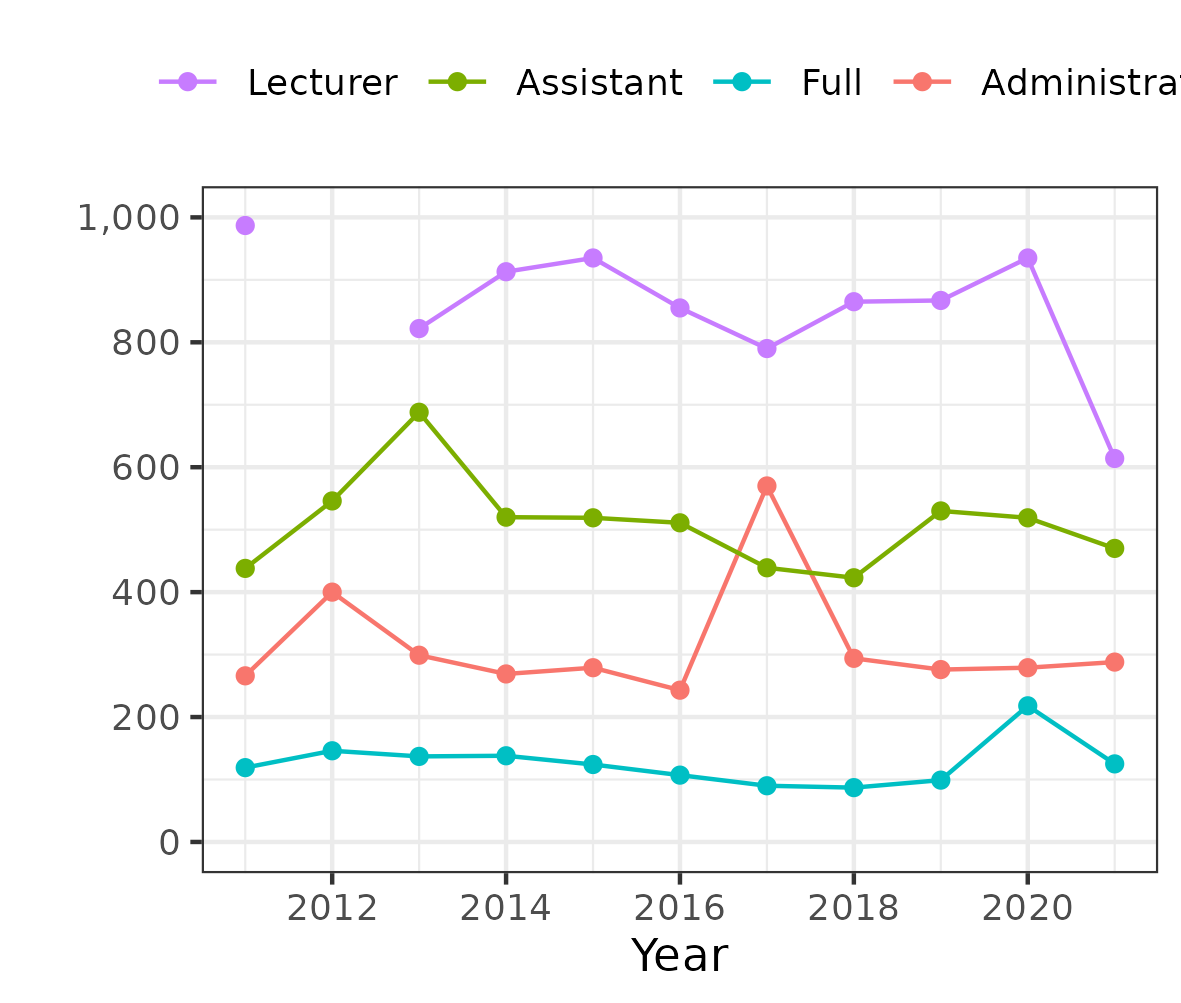
\includegraphics[width=\textwidth]{figures/newhire-count-illinois.png}
        \label{fig:newhire-count-illinois}
    \end{subfigure}
    \begin{subfigure}[b]{0.495\textwidth}
        \centering
        \caption{Mean Salary in First Year for New Hires, \$ 2021 CPI-U.}
        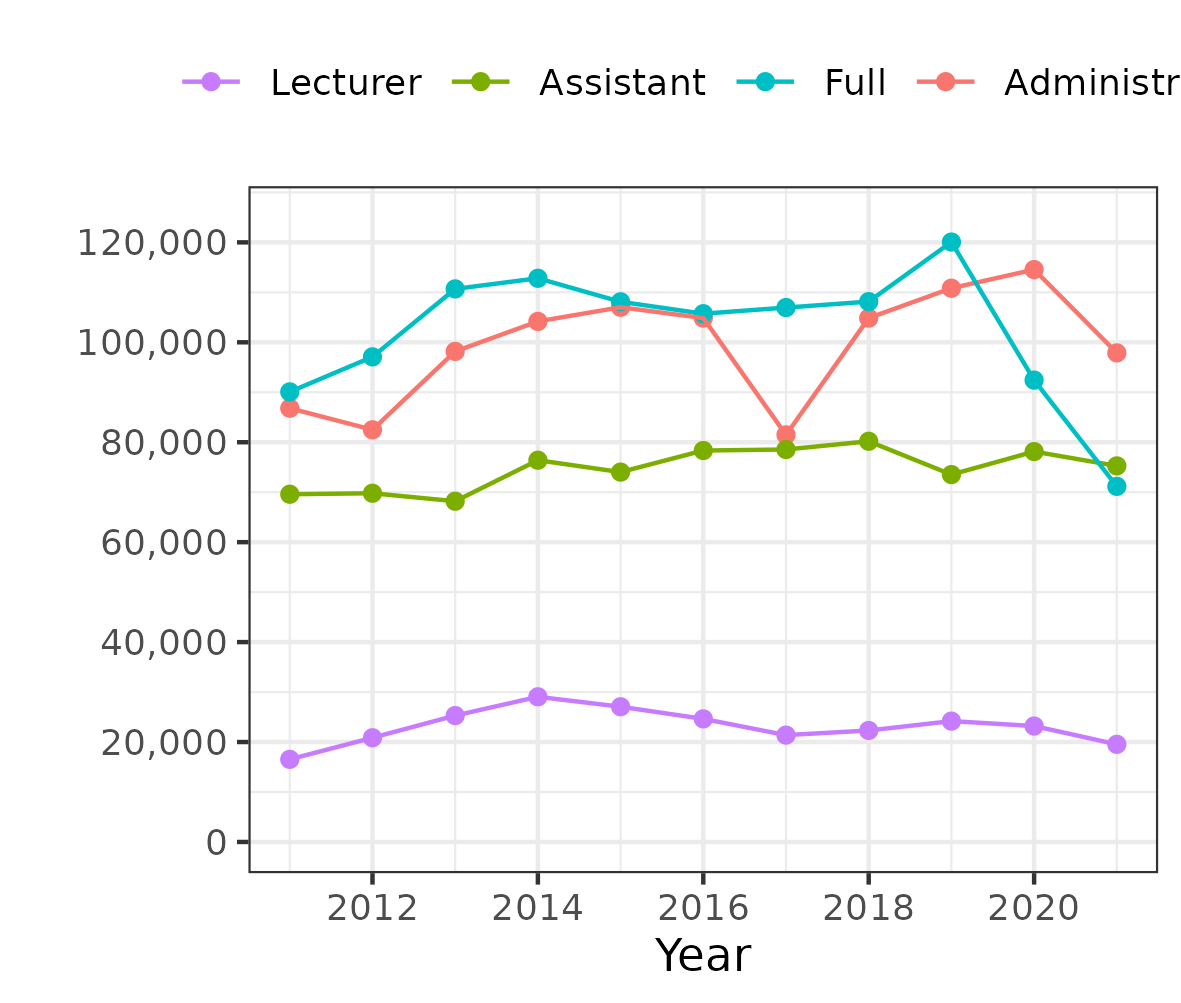
\includegraphics[width=\textwidth]{figures/newhire-salary-illinois.png}
        \label{fig:newhire-salary-illinois}
    \end{subfigure}
    \label{fig:newhire-illinois}
\end{figure}

These examples show that Illinois public universities were affected by the negative shock to state funding for higher education, and instituted policy changes aimed at affecting faculty outcomes investigated in \autoref{sec:results}.
Yet the only measurable effect was on count of professor per student (implied via slower hiring), and first-year lecturer salaries.
To investigate these trends for the entire state, \autoref{fig:newhire-illinois} shows the count of professors hired in the years 2011-2021, and their mean salary, by position.
In particular, no position had sustained rises in hiring while enrolment within the university was rising (so that new hires per student necessarily fell), and hiring of new administrators jumped once the Illinois budget crisis ended in 2017.
At the same time, professor new hires' starting salaries remained relatively constant for lecturer and assistant professors, yet rose and fell over the decade for full professors and administrators.
